\section{Monday, April 7: Model Validation and Selection}

\subsection{Some comments on the midterms}

\subsubsection{Review of common mistakes from in class midterm}
\begin{itemize}
\item \textbf{Problem 2: } Need to mention that deep learning is still subject to the bias-variance tradeoff! For a bit it seemed like double descent was going to challenge this, but recent work has shown that double descent is still governed by the same principles!
\item \textbf{Problem 3:} Recall the difference between a model and a model-fitting-procedure. A linear regression with $5$ covariates is a very simple model. We don't really need to worry about overfitting if we fit linear regression with $5$ pre-specified covariates. But, the procedure of ``search through 16,000 possible covariates and use stepwise regression to select the best $5$" is a very complex model-fitting-procedure. We definitely need to be worried about overfitting in this case! You all saw something really similar to this on a HW problem! 
\begin{itemize}
\item When we talk about bias / variance / overfitting: we are usually talking about a model-fitting-procedure: something that takes in a random training set and outputs a model. On the other hand, when we talk about interpretability or inference (coming soon!), we often want to talk about a specific model. 
\item When we talk about predictive accuracy: which do we care about? This is actually a tricky question, which does not relate to the in-class midterm but does relate to the idea of a ``model" vs. ``model fitting procedure". 
\begin{itemize}
\item If we are getting ready to ``deploy" a specific model to be used in the real world: we probably want to know the predictive accuracy of this specific model: trained on our entire training set! 
\item Unfortunately, this specific accuracy is hard to estimate! We can use cross-validation on the training set to estimate predictive accuracy. But ... this CV uses a bunch of different models fit to different subsets of the training data-- not our full final model! Tricky! 
\item Looking at the predictive accuracy of our fixed model on a large test set would be nice. But ... if we had such a large test, why wouldn't we use some of this data as training data to improve our model??
\end{itemize}	
\end{itemize}
\item \textbf{Problem 4: } In an image classification, the individual pixels are not meaningful! The patterns between the pixels are meaningful. So variable selection and additive models fundamentally don't make much sense. 
\begin{itemize}
\item Consider identical copies of the same image, but in one image everything has been shifted one pixel to the left. Any sort of model that is additive in the original features will be really bad at recognizing these two images as similar! 
\item One implication (relevant to what is coming, not the midterm): we need to think about what we mean by ``interpretable" for an image classification problem. Consider a lasso model that selects 10 pixels to be used for classification. The model is simple enough for us to see what coefficients go with which pixels. But, is it actually useful for us to know the coefficient of pixel (4,17)? How do we make sense of that? 
\end{itemize}
\item \textbf{Problem 5: } Honestly, this went pretty well. There weren't specific rows that everyone got wrong or anything. 
\begin{itemize}
\item One commonly forgotten common principle: if we have a tuning parameter like $\lambda$ in a ridge penalty or $k$ in KNN that directly controls model complexity, we know exactly what changing it will do to training error. Training error is lower for more complex models: it monotonically decreases as we move along the complexity axis! On the other hand, for test error, this tuning parameter has some ``ideal" value that depends on the true data generating mechanism! The test error curve is U-shaped! So we often don't know if it will go up or down as we move along our complexity axis! 
\end{itemize}
\item \textbf{Problem 6: } Check derivative algebra! Also, stochastic gradient descent processes training data in batches, so can be used for online learning. So, we might use stochastic gradient descent instead of the closed form solution for ridge regression if we have so much training data that we don't even want to store it in memory, or if our training data is coming to us over time.
\end{itemize}

\subsubsection{From the takehome midterm}

\begin{itemize}
\item \textbf{Problem 1:} If a proof tells you that something has expected value $c$, and then you simulate to verify your proof, as you increase the number of repetitions, you should be able to get a result that is equal to $c$ with a margin of error of $0.0000001$, and even this should shrink with the number of iterations. 
\begin{itemize}
\item Sometimes the proof will also rely on the sample size $n$ being big or something- and then you will also need to make this big in your simulation. But sometimes it does not! 
\item The empirical average difference between training error and test error should have converged to exactly $2/n p \sigma^2$ as the number of iterations increased. This did not depend on $n$, $p$, or $\sigma^2$.
\item The key thing here that was tricky: the $p$ in the expression is the number of coefficients in your regression model. So, unless you specifically told \texttt{lm()} to remove the intercept, then your effective $p$ is actually $p+1$!
\item If you happened to pick a big value of $n$, then the value of $2/n p \sigma^2$ barely changes when you change $p$ to $p+1$. So this makes this hard to spot. But, for a lot of you, I think the difference was large enough that you should have been able to spot this difference.
\end{itemize}
\item \textbf{Problem 2:} I wanted people to think carefully about exactly what they were seeing, and go beyond what they read in textbook! What the heck was elasticnet doing with those correlated variables? Was it ``good" or ``bad"? 
\item \textbf{Problem 3:} I was happy overall! And, this is basically our topic for today! So, people would do even better after today! 
\end{itemize}

\subsection{Back to regularly scheduled programming: review!}

Before spring break, we learned about so many different machine learning algorithms. We also learned about so many axis on which to compare these algorithms. Let's briefly review these, since it has been a while. This table (while really full) is not at all exhaustive! It's just to remind you of algorithms that we have seen, and some basic properties. You should be able to make a table like this yourself but fill in your own thoughts and ideas!

\begin{table}[H]
\scriptsize
\begin{tabularx}{\textwidth}{|X|X|X|X|X|X|X|}
\hline
&&&&&& \\ 
& When? & Bias? & Variance? & Usability? & Interpretability? & Efficiency? \\ 
&&&&&& \\ 
\hline 
Linear regression (no bells and whistles) & Regression & Unbiased if true model is linear; otherwise likely biased (too simple) & Likely low because simple. Not low if $p$ is really big. & Easy! & Easy! & Easy! \\
\hline 
Linear regression with engineered features (splines, polynomials, etc). & Regression, worried linear isn't good enough.  & Unbiased if you pick good features; otherwise likely biased. & Variance increases if you make engineered features really complicated (splines). Decreases if you are reducing dimension or redundancy (PCA). & Pretty easy, but you need to pick your features (how many PCs, degree of spline, etc). & Not amazing but not a black box. & Pretty good! \\
\hline
Stepwise regression.  & Regression, $p$ is really big, want to select subset.  & Unbiased if true model linear or you added nicely engineered features; biased otherwise. Fewer steps = potentially more bias (miss out on important variables). & Grows if $p$ is bigger or number of steps is bigger. So much greedy searching!& Pretty easy! Need to decide step criteria and stop criteria. & Even better! & Can seem slow, but faster than ``best subset" because greedy approximation.\\
\hline 
Lasso Regression & Regression, $p$ is really big, want to select subset. & Bias grows with $\lambda$, and might just be big if true model not linear. & Variance shrinks with $\lambda$. Never THAT bad if $p$ not too big. & I think easy! Just use CV to tune $\lambda$. & Pretty good! & Pretty good! \\ 
\hline  
Ridge regression  & Regression, $p$ is really big; want to reduce variance.  & Same as lasso. & Same as lasso. & Same as lasso. & Less interpretable than lasso. & Even better than lasso! Closed form! \\
\hline  
Logistic regression; with engineered feature, stepwise, lasso, or ridge extensions & Classification (mostly binary, but has multi-class extensions) & \multicolumn{5}{|c|}{Fill in same as all the linear regression rows.} \\
&& \multicolumn{5}{|c|}{(but now no-bias means that log-odds are linear in the included features).} \\
&& \multicolumn{5}{|c|}{(when classes are well-separated, hard to estimate log-odds in the ``in-between" area. high variance.) } \\
\hline
KNN & Regression OR classification, when you think you have non-linearity, and when $p$ is not too big. & Small if $k$ is small. & Big if $k$ is small. & Easy! Just pick $k$. Not going to work well in high dimensions, and then will need to consider PCA, etc. & Not a black box. ``Prototype" interpretation.  & Can be bad in terms of time and space without clever tricks.  \\ 
\hline 
LDA & Classification, when you think your classes are linearly separable, or, equivalently, Gaussian with shared variance. & Biased if not linearly separable & Pretty low variance. & Easy, I don't even think there is a tuning parameter. & Pretty good! & Easy!  \\
\hline
QDA & Classification when you think your classes are Gaussian with non-equal variance & \multicolumn{5}{|c|}{(Same as LDA basically, just slightly higher variance.)} \\  
\hline 
GAM & Regression. For classification, use logistic GAM. & Low bias because we let our model be really wiggly. But misses out on interactions! & Potentially high variance if we don't regularize or if we have a lot of features & Not bad, but there are a lot of moving pieces we could tweak. & Could be worse. Additive lets us make nice variable-by-variable plots. & Iterative back-fitting required; not bad.   \\
\hline 
Neural Network & Classification or regression; good for complex tasks! & SUPER LOW. Even gets all the interactions & Really high without proper regularization.  & A lot of things to fiddle with; hard to use. & Black-box. & Slow; use stochastic gradient descent.   \\
\hline 
Trees & Classification or regression. & Bias shrinks as tree depth increases. & Variance grows as tree depth increases. & Super easy, although you do need to decide on a stopping criteria, and choice can affect results & Small trees are really easy for humans to interpret. But beware instability! & Fast! \\
\hline 
Support vector machines & Mainly classification! We did not cover the regression setting. & If you use a ``high dimensional" kernel and big budget, really low bias!! & Variance increases as you make kernel higher dimensional or increase budget. & I think pretty easy to use out of the box. & Not that interpretable; I guess you can look at the weights if you are using a linear kernel & A bit slower (you might have noticed this in R!). \\
\hline 
\end{tabularx}
\end{table}

\subsection{No free lunch}

Why is it necessary to introduce so many different statistical learning approaches, rather than just a single best method? There is \emph{no free lunch}\footnote{This is the name of an actual theorem!} in statistics: no one method dominates all others over all possible data sets. On a particular data set, one specific method may work best, but some other method may work better on a different data set. Hence, it is an important task to decide for any given set of data which method produces the best results. Selecting the best approach can be one of the most challenging parts of performing statistical learning in practice.

\subsection{How we pick the best model depends on our goals!}

In the Breiman ``two cultures" reading that you will all complete for Monday, Breiman claims that there are two possible goals of statistical modeling: 
\begin{enumerate}
\item \textbf{Prediction:} Make accurate predictions for new data. 	
\item \textbf{Information:} Describe or understand something about the universe is generating the data.
\end{enumerate}
This probably is not a surprise to any of you- this is a common way to talk about two goals of predictive modeling. In the Efron reading that you will complete for Monday, Efron expands this classical list of two goals to a list with three possible goals. 
\begin{enumerate}
\item \textbf{Prediction:} Make accurate predictions for new data. 
\item \textbf{Estimation:} Learn the parameters of a model that can be written down (e.g. a regression model). 
\item \textbf{Attribution:} Formally determine which variables are important. 
\end{enumerate}
I like that Efron distinguishes between estimation and attribution. However, it is not clear exactly how Efron's three goals map to Breiman's two goals. To gain valuable information, do we need to have parameters that we are estimating? Can we gain information about the universe without doing formal attribution? Also, while I don't think it is a surprise to any of you that we will pick a different modeling approach depending on our ultimate goal, do you think that these different goals are at odds with one another? Or do you think that they can be complimentary? I look forward to hearing what you all think when I read your reading responses next week! 

For the rest of class today, let's assume that our primary goal is prediction. And let's go into a bit more depth about how to select the best model when our goal is predictive accuracy. 


\subsection{A bit more about picking models based on predictive accuracy}

First of all, it is important to note that the \emph{no free lunch} idea applies even if our goal is only predictive accuracy! 

Consider the extremely naive model that ignores the training data and always predicts $\hat{y}=3$. Well, if we happen to live in a universe where $Y = 3 + \epsilon$, and none of the covariates $X$ are important, then this model is optimal in terms of its mean squared error on new data! And the model $\hat{y} = \bar{y}_{train}$ will also do quite well. Since, we never know what the true universe data generating mechanism is, we can never say for sure that this ``intercept-only" model $\hat{y} = \bar{y}_{train}$  is worse than deep learning! 

You all already know that we can't just compare models based on their training error. If we compare models based on their training, then we will always prefer the most complex models with the highest degrees of freedom. In the example above, deep learning will certainly have lower training error than $\hat{y}=3$, because it will fit to the noise in the data. Instead, you all already know that we want to assess which models will perform the best on new, unseen data. 

Let's talk a bit more formally about how we assess expected predictive accuracy on new data. We have already touched on many of these methods/concepts, but I want to close the loop on ESL Chapter 7 because it is such an important chapter!

First, we need to mention that there are two separate things that we might be doing when we try to assess the accuracy of a model on new data. 
\begin{itemize}
\item \textbf{Model Selection:} We want to compare several models or several model-fitting-procedures to decide which one to use as our final model. 
\item \textbf{Model Evaluation:} After choosing a final model, we want to estimate its final accuracy on new, unseen data.
\end{itemize}

Most data analysis pipelines involve model selection. Thus, we usually actually want to do both of these tasks. And, when we are doing both of these tasks, we need to be careful about how we use our data! 

\subsubsection{Train / test / validate}

The gold standard way to carry out a data analysis pipeline that involves both selection and evaluation is the \textbf{train, validate, test} paradigm. The idea is simple. 
\begin{itemize}
\item We split our data into three datasets: train, validate, and test. 
\begin{itemize}
\item To compare a bunch of models, we can train them on the training set, and then we can compute their error on the validation set. We can select the model that seems to perform best on the validation set. 
\item The validation-set error of the selected model is a biased estimate of the true error of this model: we picked it specifically because it was a minimum-- it is biased downwards! 
\item So, we end by evaluating the performance of our selected model on the test set.
\end{itemize}	
\end{itemize}

However, sometimes we don't have enough data to want to split it into three parts! So, there are some other options.

\subsubsection{Fancy equations to estimate test error from training error}

One option! If we can compute or estimate the \textbf{degrees of freedom or optimism} of a model, then we know that the expected test error is related to the training error via a simple formula. Thus, we can use an equation to figure out a \textbf{bound} on the expected test error, and then select the model that seems to have a low expected test error. This eliminates the need for a validation set. This is the reason why we can reasonably select a model based on AIC, BIC, or Mallow's CP. A limitation of these methods is that they relate only to the in-sample (fixed X) prediction error: they say nothing about what might happen at new values of $X$. 

There are a couple of other ways of measuring model complexity besides degrees of freedom or optimism. One is VC dimension! Have any of you heard of VC dimension? This gives you another way to bound the difference between training error and test error. It is a pretty loose bound and we are not going to cover this!

One reason that we don't always use this option: degrees of freedom or VC dimension are very hard to compute for complex procedures!!! So ... we can't actually use these bounds!

\subsubsection{Cross Validation}

Cross validation re-uses data cleverly, and so can be more efficient than a train/test/validate split. But it is also a huge can of worms that is more complicated than it seems.  

First, note that, if we are doing both model selection and estimate predictive accuracy, we really should still separate your data into a training set and a test set. We can then use cross validation on our training set to select a model. We can then re-fit the model with the selected tuning parameter on the entire dataset, and can then evaluate this model on the test set. You have all done this on your HW, basically every time that you have used glmnet: you use \texttt{cv.glmnet} to pick $\lambda$, but you still then evaluated the prediction error on a test set.

One reason that this is important: the CV error of a model that is selected because it minimizes the CV error is biased downward! Because it is a selected minimum! This is a very important concept. 

If we are not doing any selection, and are just doing assessment, then we can get away with doing CV on our entire dataset. But, it is still conceptually tricky to figure out exactly what cross validation error is measuring! Since we fit a different model to each fold, and also each of these models only gets to use $(K-1)/K \times n$ of the data points for training, it is not exactly the same as evaluating the prediction error of a fixed model fit to $n$ observations. When we are just comparing different procedures to select a tuning parameter, we might not care about this. But when we are trying to evaluate a model, we do care! 

Figure 7.8 of ESL, which is copied below as Figure~\ref{fig_cv} shows why the number of folds could have a big impact on what cross validation is actually measuring. Cross-validation as an estimate of expected prediction error has its own bias-variance tradeoff, which depends on the number of folds used. While there is no exact rule for how to decide how many folds to use for cross validation, a good rule of thumb is 5-10.  

\begin{figure}
\centering
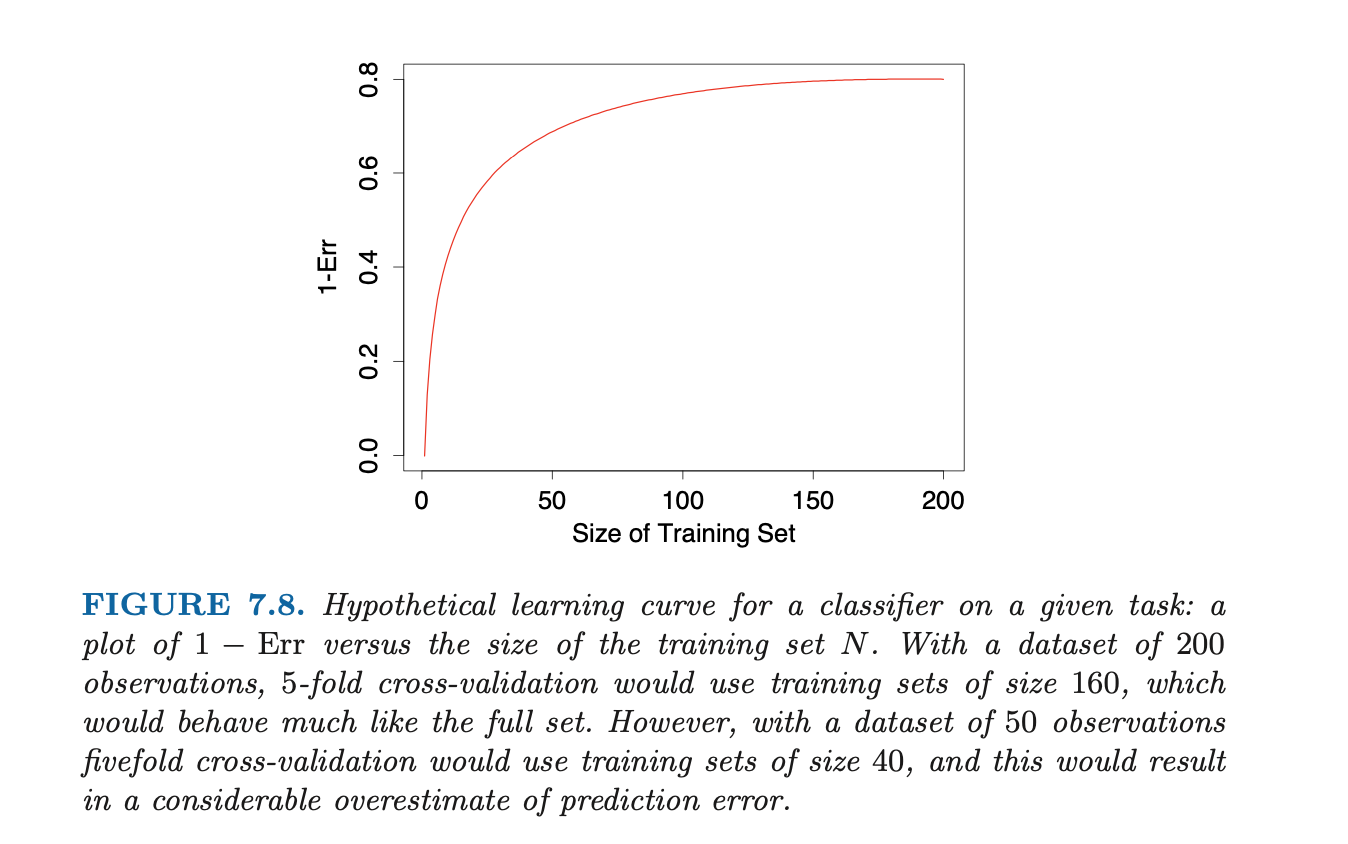
\includegraphics[width=0.6\textwidth]{442_lecs/cv_esl.png}
\caption{Figure 7.8 from ESL!}
\label{fig_cv}	
\end{figure}

You need to be really careful about making sure that model selection and model assessment are both done properly using held out data. Recall your HW problem on the wrong way to do cross validation!! And see ESL 7.10.2. The idea is that we need to use CV to evaluate an entire model-fitting procedure. We are not allowed to do any part of the procedure (i.e. variable selection) using the entire dataset-- if we do, then the test set isn't truly ``held out".

I think that this concludes our study of ESL Chapter 7, and I think you are all experts now at selecting models with good predictive accuracy! Next week, and on your HW, you will think about other things that we might want to consider when selecting a model!










